\documentclass{article}

% Gestion des polices en fonction de l'encodage (PDFLaTeX, XeLaTeX, LuaTeX ou autre) :
\usepackage{ifxetex}
\usepackage{mathtools}
\usepackage{amssymb}
\usepackage{ifluatex}
\ifxetex
  % XeTeX est utilisé :
  \usepackage{fontspec}
\else
  \ifluatex
    % LuaTeX est utilisé :
    \usepackage{fontspec}
  \else
    % pdfLaTeX ou autre moteur est utilisé :
    \usepackage[T1]{fontenc}
    \usepackage[utf8]{inputenc}
    \usepackage{lmodern}
  \fi
\fi

% Autres packages :
\usepackage[french]{babel}
\usepackage{mdframed}
\usepackage{enumitem}
\usepackage{hyperref}
\usepackage{amsmath}
\usepackage{amsfonts}
\usepackage{stmaryrd}
\usepackage[explicit]{titlesec}
\usepackage{framed}
\usepackage{amsthm}
\usepackage{xcolor}
\usepackage{tcolorbox}
\tcbuselibrary{breakable}
% Package permettant de générer des graphes :
\usepackage{tikz}
\usetikzlibrary{arrows}
\usetikzlibrary{arrows.meta}
\usepackage{pgfplots}
\pgfplotsset{compat=1.18} % Préciser la version de pgfplots afin qu'il soit compatible avec le type de cocument (ici "article").
%package pour images
\usepackage{graphicx}
\graphicspath{ {./ressources/} }


\sloppy % Pour que les URLs ne dépassent pas des marges.

\title{Algorithme d'Hasting Metropolis - Problème du voyageur de commerce}
\author{PEROTTINO Tony, VAILLANT Corentin, \\ LE BER Tom, BERNARD Léo}

% Enable SageTeX to run SageMath code right inside this LaTeX file.
% http://doc.sagemath.org/html/en/tutorial/sagetex.html
% \usepackage{sagetex}

% Enable PythonTeX to run Python – https://ctan.org/pkg/pythontex
% \usepackage{pythontex}

\begin{document}
\maketitle

\newpage
\tableofcontents
\newpage

\section*{Préambule}

Ce rapport s'inscrit dans le cadre de la matière "Projet de Mathématiques" de l'université de Toulouse (Paul Sabatier). \\
L'objectif de ce rapport est de présenter et de prouver l'algorithme d'Hastings-Metropolis. À la fois d'expliquer en détail son fonctionnement, mais aussi de comprendre l'intérêt qu'il présente dans les sciences et en quoi il prend sa valeur. \\
Pour illustrer l'algorithme, nous nous intéresserons au problème du voyageur de commerce et étudierons sa complexité.


\section{Introduction}

Afin de comprendre en profondeur ce sujet, il est nécessaire de s'en faire une idée globale, même naïve, pour pouvoir suivre convenablement la ligne directrice de notre discours.

\subsection{Informations générales et description historique}

L'algorithme d'Hastings-Metropolis consiste en une méthode d'échantillonnage stochastique permettant, à partir d'une distribution de probabilité donnée, de pouvoir décrire son comportement et d'obtenir des statistiques dessus. Cet algorithme prend sa valeur quand la distribution est difficile à analyser (systèmes multidimensionnels, par exemple). Cette méthode est marquante, car elle a été conceptualisée tôt dans l'histoire de l'informatique et a mis des décennies avant d'être prouvée et expliquée entièrement. \\
C'est en 1949 que l'écriture de l'algorithme a été publiée dans un article de Nicholas Metropolis et Stanisław Ulam. La paternité de l'algorithme est soumise à débat, car l'algorithme s'inscrit sous le nom de son chef de projet (Metropolis), alors que l'équipe composée de Nicholas Metropolis, Arianna et Marshall Rosenbluth, Augusta et Edward Teller a contribué à cette méthode. Ils étudiaient alors plus particulièrement le cas de la distribution de Boltzmann, une des distributions les plus utilisées en physique statistique, dans des travaux datant de 1953. \\
Cela illustre une dynamique fréquente dans les sciences, où le mérite est disproportionnellement attribué à une personne alors qu'il s'agit des efforts de toute une équipe. En particulier, Arianna Rosenbluth était considérée comme brillante par le monde scientifique. \\

En 1970, W. K. Hastings (1930-2016) a étendu l'algorithme au cas d'une distribution quelconque, et c'est cette version généralisée qui est connue sous le nom d'algorithme de Metropolis-Hastings. Cette extension a eu de nombreuses applications dans divers domaines scientifiques, comme en statistique bayésienne (espaces complexes multidimensionnels), en biologie computationnelle (analyse des séquences génétiques), en économie et en finance (modèles stochastiques MCMC en général), etc. \\

Quant à lui, le problème du voyageur de commerce (dit "TSP", comme Travelling Salesman Problem en anglais) est un problème classique et bien connu pour être un problème NP-difficile et NP-complet, ce qui signifie qu'il est extrêmement difficile de trouver une solution optimale en temps polynomial, et il est peu probable que des algorithmes en temps polynomial existent pour résoudre ce problème de manière exacte. \\
L'origine du problème est assez incertaine : il a été formulé pour la première fois vers 1850 dans un manuel d'un commerçant voyageant en Suisse et en Allemagne. Ce n'est que dans les années 1930 que le problème fut énoncé d'abord comme un casse-tête (par William Rowan et Thomas Kirkman), puis étudié (par, entre autres, Thomas Kirkman, Jillian Beardwood, J. H. Halton et John Hammersley). \\ 
Le problème consiste à déterminer le chemin le plus court passant par tous les points d'un graphe une seule fois chacun, en terminant par le point de départ (recherche d'un cycle hamiltonien le plus court). Les distances peuvent être dites symétriques ou asymétriques, c'est-à-dire que la distance entre eux varie en fonction de la direction du déplacement. On peut illustrer ce problème grâce à un voyageur de commerce devant vendre ses produits dans chacune des villes en un minimum de temps. Ce problème peut donc être naturellement représenté par un graphe.\\

% Insérer une image ! % Pouquoi il est là ce commentaire ?

\subsection{Pourquoi HM permet-il de résoudre le problème du voyageur de commerce ?}

Le principe mathématique derrière HM repose sur la construction dynamique d'une chaîne de Markov, qui n'est pas connue au préalable mais se développe au fil des itérations. À mesure que l'algorithme progresse, le comportement de cette chaîne converge vers la distribution cible, permettant d'obtenir un échantillon fiable par rapport aux états de la distribution. \\
Quant au problème du voyageur de commerce, il peut être représenté par un graphe orienté ayant un sommet pour chaque ville et une arête pour chaque temps de trajet. Nous verrons par la suite qu'une chaîne de Markov peut être associée à un graphe orienté, c'est-à-dire que le problème du voyageur de commerce est résoluble par HM. \\

De plus, nous avons précisé au préalable que le voyageur de commerce était NP-difficile et NP-complet. En conséquence, l'objectif de HM n'est pas d'apporter la réponse exacte au problème, mais une approximation fidèle de la solution, ce qui peut sembler contre-intuitif. Cette approximation est la caractéristique principale des méthodes MCMC que nous aborderons dans leur partie dédiée. \\
Plus généralement, il faut donc comprendre que HM est un outil adapté à la résolution de problèmes ayant un trop grand nombre de possibilités pour être explorées toutes dans un temps raisonnable. C'est pour cela que la résolution de ces problèmes se fait par l'approximation de la bonne solution (en étudiant donc des échantillons de toutes les possibilités). \\
Cette nuance est très importante, car elle révèle en quoi HM est un outil sophistiqué. \\ 

\subsection{Objectif de ce rapport}

Il est donc compréhensible que, pour prouver HM, nous allons devoir tout d'abord comprendre le fonctionnement des chaînes de Markov et en expliciter les définitions fondamentales, puis leur comportement sur le temps long, pour pouvoir ensuite construire la preuve mathématique derrière HM et déterminer les raisons de son fonctionnement. Nous étudierons à la fois cette preuve et ferons un détour par les méthodes MCMC (Monte-Carlo), dont HM est issu. Nous finirons par conclure ce rapport avec une implémentation personnelle de HM pour illustrer nos propos.



\newpage
\section{Chaînes de Markov à états finis}

\subsection{Définitions fondamentales}

% TODO = Parler des définitions et surtout placer le contexte, j'entends par là :
% - [X] En mathématiques, une chaîne de Markov est un processus de Markov à temps discret, ou à temps continu et à espace d'états discret. Un processus de Markov est un processus stochastique possédant la propriété de Markov : l'information utile pour la prédiction du futur est entièrement contenue dans l'état présent du processus et n'est pas dépendante des états antérieurs (le système n'a pas de « mémoire »).
% - [X] Dixit Wikipedia "\url{https://fr.wikipedia.org/wiki/Chaîne_de_Markov}", j'entends par là définir "temps discret/continu", "processus stochastique", etc.

\begin{tcolorbox}[colback=white,colframe=blue!80!black,title=Temps Discret et Temps Continu]
Soit $T$ un ensemble d'indices numérotées représentant le temps. \\

Il existe deux types de modélisation temporelle :
\begin{enumerate}[leftmargin=5em, label=(\arabic*)]
    \item Un processus \textbf{à temps discret} signifie que l'on considère les valeurs de la modélisation comme espacées régulièrement dans le temps.
          On peut prendre des ensembles dénombrables comme $T = \mathbb{N}$ ou $T = \mathbb{Z}$ où chaque instant est distinct.
    \item Un processus \textbf{à temps continu} signifie que $T$ n'est pas dénombrable. Il existe toujours un temps intermédiaire entre deux indices de $T$.
          Cela signifie que le processus évolue en tout instant dans un continuum temporel, on peut prendre des ensembles non dénombrables comme $T = \mathbb{R}_+$ où chaque instant est continu.
\end{enumerate}
\end{tcolorbox}

Dans ce rapport nous nous interesserons uniquement au temps discret, pour pouvoir modéliser le problème du voyageur de commerce.
De plus, cette distinction joue un rôle fondamental dans la classification et l'analyse des \textbf{processus stochastiques} et n'implique pas les mêmes théorèmes. \\

\begin{tcolorbox}[colback=white,colframe=blue!80!black,title=Processus Stochastique]
Soit $(\Omega, \mathcal{F}, \mathbb{P})$ un espace de probabilité.

Soit $T$ un ensemble d'indices discret ou continu (souvent $T = \mathbb{N}$ ou $\mathbb{R}_+$). \\

Un \textbf{processus stochastique} est une famille de variables aléatoires $\{X_t\}_{t \in T}$ définies sur $(\Omega, \mathcal{F}, \mathbb{P})$ et à valeurs dans un espace d'états $E$ (appelé espace d'états du processus).
\end{tcolorbox}

Un processus stochastique permet de modéliser un système évoluant de manière aléatoire en fonction du temps.

Différents types de processus peuvent être étudiés en fonction des propriétés de dépendance temporelle et de la nature de l'espace d'états $E$.
Au cours de ce rapport, nous nous concentrerons l'un des principaux processus stochastiques à temps discret et à espace d'états fini ; les \textbf{chaînes de Markov}. \\

\begin{tcolorbox}[colback=white,colframe=red!80!black,title=Chaîne de Markov]
Soit $E$ un ensemble fini ou dénombrable.

Soit $(X_n)_{n \in \mathbb{N}}$ une suite de variables aléatoires à valeurs dans l'espace d'états $E$. \\

$(X_n)_{n \in \mathbb{N}}$ est appellée \textbf{chaîne de Markov} si et seulement si :
\begin{enumerate}[leftmargin=5em, label=(\arabic*)]
    \item Sa loi de probabilité initiale $X_0$ est bien définie.
    \item Elle respecte la \textbf{propriété de Markov}, telle que :
\end{enumerate}
\[
\forall n \geq 0, \quad \exists x_1, x_2, \dots, x_{n+1} \in E,
\]
\[
\mathbb{P}(X_{n+1} = x_{n+1} \mid X_1 = x_1, \dots, X_n = x_n) = \mathbb{P}(X_{n+1} = x_{n+1} \mid X_n = x_n).
\]
\end{tcolorbox}

Une chaîne de Markov est un processus de Markov à temps discret ou à temps continu et à espace d'états discret. Un processus de Markov est un processus stochastique possédant la propriété de Markov : l'information utile pour la prédiction du futur est entièrement contenue dans l'état présent du processus et n'est pas dépendante des ses états antérieurs.

Autrement dit, la loi de probabilité $\mathbb{P}$ régissant la transition de l'état présent $X_n$ vers l'état futur $X_{n+1}$ dépend uniquement du dernier terme $X_n$, et reste totalement indépendante des tous ses états antérieurs $\{X_0, X_1, \dots, X_{n-1}\}$.

Cette propriété, que l'on peut qualifier de « sans mémoire » ou de propriété de Markov, constitue la caractéristique fondamentale de ces processus stochastiques.

\begin{tcolorbox}[colback=white,colframe=blue!80!black,title=Chaine de Markov Homogène]
Un chaine de Markov est dite homogène quand $\forall n \in \mathbb{N}$ :
\[
  \mathbb{P}[X_{n+1} = j \mid X_n = i] = \mathbb{P}[X_1 = j \mid X_0 = i].
\]
\end{tcolorbox}

En somme, une chaîne de Markov homogène ne dépend pas des états précédents (propriété de Markov) et garantit que son comportement reste inchangé au fil du temps, c'est-à-dire que les probabilités de transition restent constantes quelque doit $t \in T$ (homogénéité de la chaine de Markov). \\
Dans ce rapport, toutes les chaînes de Markov seront considérées comme homogènes.

\newpage
\subsection{Propriétés fondamentales}

% TODO
% Propriétés à parler : 
% - [X] Matricer de transition
% - [X] Lien avec les graphes orientés
% - [X] Propriétés en n-pas

\subsubsection{Matrice de Transition}

\begin{tcolorbox}[colback=white,colframe=red!80!black,title=Matrice de Transition]
Soit $(X_n)_{n \in \mathbb{N}}$ une chaîne de Markov homogène à valeurs dans un ensemble fini ou dénombrable $E$.

Soit la famille de nombres réels $(X_n)_{n \in \mathbb{N}}$ permettant de passer d'un état à un autre, définie comme :
\[
\forall n \geq 0,\; \forall i,j \in E,\quad P_{ij} = \mathbb{P}(X_{n+1} = j \mid X_n = i).
\]

La \textbf{matrice de transition} $P$ regroupe ces probabilités tel que chaque élément $P_{ij}$ représente la probabilité de passer de l'état $i$ à l'état $j$ en une seule étape.
Lorsque l'ensemble des états $E$ est discret, par exemple $E = \{1, 2, \dots, N\}$, la matrice s'exprime sous la forme suivante :
\[
P = \begin{bmatrix}
P_{11} & P_{12} & \cdots & P_{1N}\\[1mm]
P_{21} & P_{22} & \cdots & P_{2N}\\[1mm]
\vdots & \vdots & \ddots & \vdots\\[1mm]
P_{N1} & P_{N2} & \cdots & P_{NN}
\end{bmatrix}
\]

\end{tcolorbox}

\begin{tcolorbox}[colback=white,colframe=blue!80!black,title=Matrice stochastique par lignes/colonnes]
Une matrice \textbf{stochastique par lignes} (appelée aussi \textbf{stochastique à droite}) est une matrice dont la somme des probabilités de ses lignes vaut 1 chacune et toutes ses probabilités sont positives :
\[
\forall i, \quad \sum_{j=1}^{N} P_{ij} = 1 \quad \text{et} \quad 0 \leq P_{ij} \leq 1.
\]

Respectivement, une matrice est \textbf{stochastique par colonnes} (dite aussi \textbf{stochastique à gauche}) lorsque :
\[
\forall j, \quad \sum_{i=1}^{N} P_{ij} = 1 \quad \text{et} \quad 0 \leq P_{ij} \leq 1.
\]
Une matrice est dite \textbf{bistochastique} lorsqu'elle est à la fois stochastique par lignes et par colonnes.
\end{tcolorbox}

Dans le cadre des chaines de Markov homogènes, toutes les matrices de transition $P$ sont stochastiques par lignes car les probabilités de transition depuis chaque état sont normalisées (chaque ligne représentant le vecteur des probabilités de transition depuis un état donné vers l’ensemble des autres états). C'est-à-dire que la somme des probabilités pour passer d'un état à un autre vaut 1. \\

De manière analogue, si l'espace des états est infini dénombrable (par exemple $E = \{1, 2, 3, \dots\}$), on indexe les états de la même façon et la condition
\[
\forall i \in E, \quad \sum_{j \in E} P_{ij} = 1,
\]
reste valable.

\subsubsection{Représentation sous forme de Graphe Orienté}
\label{subsubsec: Représentation sous forme de graphe orienté}

\begin{tcolorbox}[colback=white,colframe=red!80!black,title=Graphe Orienté d'une Chaîne de Markov]
Une chaîne de Markov homogène peut toujours être représentée sous forme d'un graphe orienté $ G = (V, A) $, où :
\begin{enumerate}[leftmargin=5em, label=(\arabic*)]
    \item $ V $ est l'ensemble des sommets, correspondant aux états de l'espace d'états $ E $.
    \item $ A $ est l'ensemble des arcs, où chaque arc possède une pondération correspondant à la probabilité de transition $P_{i,j}$. Un arc de $i$ vers $j$ est représenté que si $P_{i,j} > 0$.
\end{enumerate}
\end{tcolorbox}

Représenter graphiquement une chaîne de Markov homogène permet de clarifier visuellement les différentes dynamiques de transitions entre chaque état du système et de comprendre la structure du processus stochastique. \\

\begin{tcolorbox}[colback=white,colframe=yellow!80!black,title=Exemple, breakable]
Considérons par exemple une chaîne de Markov ayant trois états $\alpha, \beta, \gamma$, ordonnés respectivement, et dont la matrice de transition est donnée par :

\begin{center}
$
P = \begin{bmatrix}
0.1 & 0.4 & 0.5 \\
0.6 & 0.4 & 0 \\
0.1 & 0.1 & 0.8 \\
\end{bmatrix}
$
\end{center}

Dans cette configuration, la probabilité de transition de l'état $\alpha$ vers l'état $ \beta $ est donnée par :
\[
P_{\alpha,\beta} = P_{1,2} = \mathbb{P}(X_{n+1} = \beta \mid X_n = \alpha) = 0.4.
\]

\newpage % /!\ TEMPORAIRE /!\ - Pour une bonne mise en page de l'exemple.
Nous obtenons ainsi le graphe suivant :

\begin{center}
\begin{tikzpicture}[
    >={Latex[length=3mm, width=2mm]},
    node distance=2cm,
    state/.style={circle, draw, minimum size=0.5cm, font=\large},
    every edge/.append style={draw, -latex, font=\small}
]

% Nodes :
\node[state] (A) at (0, 0) {$\alpha$};
\node[state] (B) at (2, 3) {$\beta$};
\node[state] (C) at (4, 0) {$\gamma$};

% Edges :
\draw[->] (A) edge[loop left, out=150, in=210, looseness=8] node[left] {0.1} (A);
\draw[->] (A) edge[bend right=20] node[left] {0.4} (B);
\draw[->] (A) edge[bend right=16] node[below] {0.5} (C);

\draw[->] (B) edge[bend right=20] node[left] {0.6} (A);
\draw[->] (B) edge[loop above, out=60, in=120, looseness=8] node[above] {0.4} (B);

\draw[->] (C) edge[bend right=16] node[below] {0.1} (A);
\draw[->] (C) edge[bend right=20] node[right] {0.1} (B);
\draw[->] (C) edge[loop right, out=330, in=30, looseness=8] node[right] {0.8} (C);

\end{tikzpicture}
\end{center}
\end{tcolorbox}

\subsubsection{Matrice de transition en \texorpdfstring{$k$}{k}-pas} % Pour que "hyperref" supporte l'expression mathématique "$k$" dans la chaîne de caractère générant un des signets du PDF.
\label{subsubsec: Matrice de transition en k-pas}

\begin{tcolorbox}[colback=white,colframe=red!80!black,title=Matrice de transition pour $k$-transitions]
Soit $(X_n)_{n \in \mathbb{N}}$ une chaine de Markov homogène d'espace d'états $E$ fini ou dénombrable tel que $\left\{1,2,\ldots,N\right\}$. On note $P$ sa matrice de transition. \\

Pour tout état $E_i$ et $E_j$ et pour tout entier naturel $k \geq 1$, le coefficient de la ligne $i$ et de la colonne $j$ de \textbf{la matrice $P^k$ est la probabilité de passer de l'état $E_i$ à celui $E_j$ en $k$ transitions}.
\end{tcolorbox}

Les chaînes de Markov homogènes permettent de déterminer l'état d'un système après $k$ transitions, c'est-à-dire au bout du $k$-ième mouvement dans la chaine, en élevant la matrice de transition à la puissance $k$. \\
Plus formellement, on a :
\[
P_{i,j}^{(k)} = \mathbb{P}(X_k = j \mid X_0 = i).
\]
Ce résultat vient de la propriété de Markov, qui indique que la probabilité de transition d'un état $i$ à un état $j$ dépend uniquement du dernier pas réalisé, et non de tous les précédents.

\begin{tcolorbox}[colback=white,colframe=green!80!black,title=Démonstration]
La démonstration de cette propriété passe par celle de l'\textbf{équation de Chapman-Kolmogorov}, telle que $\forall i,j \in E$ et $\forall n,m \in \mathbb{N}$ :
\[
\mathbb{P}(X_{n+m} = j \mid X_0 = i) = \sum_{k \in E} \mathbb{P}(X_{m} = j \mid X_0 = k) \cdot \mathbb{P}(X_n = k \mid X_0 = i).
\]

Ce qui équivaut en termes matriciels :
\[
P_{i,j}^{(n+m)} = \sum_{k \in E} P_{i,k}^{(n)} \cdot P_{k,j}^{(m)}.
\]

Cette relation peut s'interpréter en disant que pour passer de $i$ à $j$ en $n+m$ étapes il a fallu en $n$ étapes aller de $i$ à un certain $k$ puis en $m$ étapes aller de $k$ à $j$. \\

On reconnait alors l'expression de l'associativité du produit matriciel tel que :
\[
P^{n+m} = \underbrace{P \cdot \ldots \cdot P}_\textit{n fois} \cdot \underbrace{P \cdot \ldots \cdot P}_\textit{m fois} = P^{n}P^{m}.
\]
\end{tcolorbox}

\begin{tcolorbox}[colback=white,colframe=yellow!80!black,title=Exemple, breakable]
Reprenons par exemple la matrice $P$ donnée dans la sous-section~\ref{subsubsec: Représentation sous forme de graphe orienté} ci-dessus, la matrice de transition en $5$ étapes, nommée $P^{5}$, représente l'ensemble des probabilités permettant de passer de chaque état $i$ à un état $j$ au bout d'exactement $5$ étapes :
\begin{center}
$
P^{5} = \begin{bmatrix}
0,22350 & 0,24385 & 0,53265 \\
0,24150 & 0,26140 & 0,49710 \\
0,20595 & 0,22252 & 0,57153 \\
\end{bmatrix}
$
\end{center}
Toujours en reprennant notre exemple, la probabilité de passer de l'état $\alpha$ à l'état $\beta$ au bout d'exactement $5$ étapes est donc de :
\[
P_{\alpha,\beta}^{(5)} = \mathcal{P}_\alpha(\beta)^{5} = 24,385\%
\]
\end{tcolorbox}

\newpage
\subsection{Classes d'équivalence}

\subsubsection{Classification des états}
\label{subsubsec: Les différents types d'états}

Dans une chaîne de Markov, chaque état peut être classifié en différentes catégories en fonction de ses liaisons avec les autres états. Ces différentes classifications nous permettrons d'analyser le comportement de la chaîne en temps long.

\begin{tcolorbox}[colback=white,colframe=red!80!black,title=Accessibilité et communication]
Soient $i$ et $j$ deux éléments de $E$. On dit que $j$ est \textbf{accessible} à partir de $i$ si :
\[
\exists n \geq 1, \quad P_{i,j}^{(n)} > 0.
\]
Ce que l'on note $i \to j$. \\

On dit que les deux états $i$ et $j$ \textbf{communiquent} si $i \rightarrow j$ et $j \rightarrow i$. On a ainsi :
\[
\exists n \geq 0, \quad P_{i,j}^{(n)} > 0 \quad \text{et} \quad \exists m \geq 0, \quad P_{j,i}^{(m)} > 0.
\]
Ce que l'on note $i \leftrightarrow j$.
\end{tcolorbox}

En particulier, $i \to j$ si et seulement s'il existe une suite d'états $(i_0, i_1, \dots, i_n)$ avec $i_0 = i$ et $i_n = j$ telle que :
\[
P(X_n = j, \dots, X_1 = i_1 \mid X_0 = i) = P(i_{n-1}, j) \cdots P(i, i_1) > 0.
\]
Ce qui veut dire qu'il existe un chemin de probabilité strictement positive qui mène de i à j.

\begin{tcolorbox}[colback=white,colframe=blue!80!black,title=État récurrent/transitoire]
Un état $i$ est dit \textbf{récurrent} si, en partant de cet état, ill est certain d'y retourner.
Autrement dit, en effectuant un nombre infini de transitions, on retourne à $i$ une infinité de fois.

Plus rigoureusement, cela signifie que :
\[
\mathbb{P}_i(\text{Num}_i(X) = \infty) = 1,
\]
où  
\[
\text{Num}_i(X) = |\{n \geq 0 \mid X_n = i\}|
\]
représente le nombre total de visites de l'état $i$, y compris la première.

Un état qui n'est pas récurrent est dit \textbf{transient} ou \textbf{transitoire}.
\end{tcolorbox}

\begin{tcolorbox}[colback=white,colframe=blue!80!black,title=État absorbant/évanescent]
Un état $i$ est appelé \textbf{absorbant} si, une fois atteint, la chaîne reste dans cet état avec probabilité 1. Formellement, cet état satisfait :
\[
P_{i,i} = 1 \quad \text{et} \quad \forall j \neq i, \quad P_{i,j} = 0.
\]
A l'inverse, tout état ne respectant pas cette condition est appelé état \textbf{non-absorbant} ou encore état \textbf{évanescent}.
\end{tcolorbox}

\begin{tcolorbox}[colback=white,colframe=blue!80!black,title=État périodique/apériodique]
Un état $i$ est dit \textbf{périodique} si la chaîne ne peut revenir à cet état qu'après un nombre d'étapes multiple (un certain entier $d > 1$), appelé la période de $i$. La période $d(i)$ est définie comme :
\[
d(i) = \text{PGCD}\{n \geq 1 \mid P_{i,i}^{(n)} > 0\}.
\]
Si $d(i) = 1$, l'état $i$ est dit \textbf{apériodique}, ce qui signifie qu'il est possible de revenir à cet état à chaque nouvelle transition /  sans contrainte de périodicité.
\end{tcolorbox}

% Est-ce qu'il faudrait ajouter le dernier type d'état suivant ? Il est super pratique dans notre cas mais ces notions ne sont pas encore introduites à ce niveau... - Tom
% Un dernier type d'état que nous étudierons est le type ergotique.
% Un état $i$ est dit \textbf{ergodique} si, en plus d'être récurrent, il est apériodique et appartient à une classe de communication contenant tous les autres états de la chaîne.
% Les états ergodiques permettent à la chaîne de converger vers une distribution stationnaire.
% TODO A AJOUTER APRES

\subsubsection{Classes de communication}

\begin{tcolorbox}[colback=white,colframe=red!80!black,title=Classe de communication]
Soit deux états communicants $i$ et $j$. Selon la définition précédente, on a que $\leftrightarrow$ est une relation d'équivalence. De plus dans le contexte des chaines de Markov, ces classes d'équivalences sont appelées \textbf{classes de communications}.
Une classe de communication est donc un ensemble d'états accessibles les uns depuis les autres.
\end{tcolorbox}

\begin{tcolorbox}[colback=white,colframe=green!80!black,title=Démonstration, breakable]
Montrons que la relation $\leftrightarrow$ est une relation d'équivalence. \\

Il nous suffit alors de vérifier les trois propriétés suivantes :
\begin{enumerate}
    \item \textbf{Réflexivité} : Pour tout état $i \in E$, $i \leftrightarrow i$. \\
        Pour tout état $i \in E$, il existe trivialement un chemin $i \to i$. En effet, en considérant le chemin de longueur zéro (via le fait que $P_{ii}^{(0)} = 1$ en définissant $P^{(0)}$ comme la matrice identité), on conclut directement que $i \leftrightarrow i$.
\newpage % /!\ TEMPORAIRE /!\ - Pour une bonne mise en page de la démonstration.
    \item \textbf{Symétrie} : Si $i \leftrightarrow j$, alors $j \leftrightarrow i$. \\
        Si $i \leftrightarrow j$, par définition il existe un chemin $i \to j$, (et inversement un chemin de $j \to i$). Ainsi, la relation est symétrique : $i \leftrightarrow j \Rightarrow j \leftrightarrow i$.
    \item \textbf{Transitivité} : Si $i \leftrightarrow j$ et $j \leftrightarrow k$, alors $i \leftrightarrow k$. \\
    Supposons que $i \leftrightarrow j$ et $j \leftrightarrow k$. En composant ces deux chemins, on obtient un chemin $i \to k$. De manière analogue, la composition des chemins $k \to j$ et $j \to i$ nous fournit un chemin $k \to i$. Ainsi, $i \leftrightarrow k$. \\
\end{enumerate}

Comme la relation $\leftrightarrow$ satisfait les propriétés de réflexivité, de symétrie et de transitivité, elle est bien une relation d'équivalence sur $E$. Les classes d'équivalences ainsi obtenues sont allors appelées \textbf{classes de communication}.
\end{tcolorbox}

L'ensemble des classes de communication, engendrées par $\leftrightarrow$, d'une chaîne de Markov sont \textbf{disjointes} et forment une \textbf{partition} de l'ensemble des états de cette chaîne.
Autrement dit, la relation d'équivalence $\leftrightarrow$ partitionne l'ensemble des états d'une chaîne de Markov en classes de communication disjointes. \\

Les classes de communcation peuvent parfois partager les propriétés énoncées dans la partie \ref{subsubsec: Les différents types d'états} dont les définitions s'élargissent alors à la classe entière (et donc aux sous-ensemble d'états de cette classe). Il existe alors une propriété structurelle commune entre les états, que l'on appelle \textbf{propriété de classe}. \\

\begin{tcolorbox}[colback=white,colframe=blue!80!black,title=Qualificatif ouvert/fermé pour une classe de communication]
Une classe de communication appartienent systématiquement à l'une des deux catégories suivantes :
\begin{itemize}
    \item \textbf{Fermée} : Une fois qu'un état de cette classe est atteint, il est impossible de quitter cette classe. Formellement, pour une classe $C$, cela signifie que :
        \[
        \forall i \in C, \quad \forall j \notin C, \quad \forall n \geq 1, \quad P_{i,j}^{(n)} = 0.
        \]
    \item \textbf{Ouverte} : L'opposée de fermée ; il existe au moins un état de la classe qui permet de sortir de celle-ci. Plus formellement, cela signifie que :
        \[
        \exists i \in C, \quad \exists j \notin C, \quad \exists n \geq 1, \quad P_{i,j}^{(n)} > 0.
        \]
\end{itemize}
\end{tcolorbox}

L'intérêt de ces distinctions est de diviser les chaînes de Markov en sous-ensembles analytiquement indépendants, ce qui permet ensuite de tirer des conclusions sur les sous-ensembles présentant ces propriétés. \\

\begin{tcolorbox}[colback=white,colframe=yellow!80!black,title=Exemple, breakable]
Prenons par exemple la chaîne de Markov suivante, dont la représentation sous forme de graphe orienté est donnée ci-dessous :

\begin{center}
    \begin{tikzpicture}[
        >={Latex[length=3mm, width=2mm]},
        node distance=2cm,
        state/.style={circle, draw, minimum size=0.7cm, font=\small},
        every edge/.append style={draw, -latex, font=\small}
    ]
    
    % -- Position des noeuds --
    \node[state] (1) at (0,2)   {1};
    \node[state] (2) at (2,2)   {2};
    \node[state] (3) at (4,2)   {3};
    \node[state] (4) at (6,2)   {4};
    \node[state] (5) at (0,0)   {5};
    \node[state] (6) at (2,0)   {6};
    \node[state] (7) at (4,0)   {7};
    
    % -- Position des arcs --
    % 1 -> 1 :
    \draw[->] (1) edge[loop above, out=60, in=120, looseness=8]
        node[above] {} (1);

    % 4 -> 4 :
    \draw[->] (4) edge[loop above, out=60, in=120, looseness=8]
    node[above] {} (4);

    % 7 -> 7 :
    \draw[->] (7) edge[loop below, out=-120, in=-60, looseness=8]
    node[below] {} (7);

    % 1 -> 2 :
    \draw[->] (1) edge[bend left=25]
        node[left] {} (2);

    % 2 -> 1 :
    \draw[->] (2) edge[bend left=25]
        node[left] {} (1);

    % 3 -> 2 :
    \draw[->] (3) edge[bend left=25]
        node[left] {} (2);

    % 3 -> 4 :
    \draw[->] (3) edge[bend left=25]
        node[left] {} (4);

    % 4 -> 3 :
    \draw[->] (4) edge[bend left=25]
        node[left] {} (3);

    % 1 -> 5 :
    \draw[->] (1) edge[bend left=25]
        node[left] {} (5);

    % 5 -> 1 :
    \draw[->] (5) edge[bend left=25]
        node[left] {} (1);

    % 2 -> 6 :
    \draw[->] (2) edge[bend left=25]
        node[left] {} (6);

    % 3 -> 7 :
    \draw[->] (3) edge[bend left=25]
    node[left] {} (7);

    % 5 -> 6 :
    \draw[->] (5) edge[bend left=25]
        node[left] {} (6);

    % 6 -> 5 :
    \draw[->] (6) edge[bend left=25]
        node[left] {} (5);
    
    % -- Encadrement des classes (avec bord arrondis) --
    % Classe 1 = {1, 2, 5, 6} :
    \draw[rounded corners=5pt, thick, red!80!black] (-0.5, 2.5) rectangle (2.5, -0.5);

    % Classe 2 = {3, 4} :
    \draw[rounded corners=5pt, thick, red!80!black] (3.5, 2.5) rectangle (6.5, 1.5);

    % Classe 3 = {7} :
    \draw[rounded corners=5pt, thick, red!80!black] (3.5, 0.5) rectangle (4.5, -0.5);

    \end{tikzpicture}
\end{center}

Dans cette chaîne de Markov, nous avons trois classes de communication :
\begin{itemize}
    \item La classe 1, formée par les états $\{1, 2, 5, 6\}$.
    \begin{itemize}
        \item Cette classe est fermée car il n'est pas possible de quitter cette classe une fois qu'un état de celle-ci est atteint. En effet, il n'existe pas d'état $j$ tel que $P_{i,j} > 0$ pour $i \in \{1, 2, 5, 6\}$ et $j \notin \{3, 4, 7\}$.
\newpage % /!\ TEMPORAIRE /!\ - Pour une bonne mise en page de l'exemple.
        \item Chaque état de la classe est alors récurrent car il est certain de revenir à un des états $i \in \{1, 2, 5, 6\}$ après un nombre infini de transitions.
    \end{itemize}
    \item La classe 2, formée par les états $\{3, 4\}$.
    \begin{itemize}
        \item Cette classe est ouverte car il est possible de la quitter via $3 \to 2$ et $3 \to 7$.
        \item Chaque état de la classe est alors transitoire car nous ne reviendrons pas aux états $i \in \{3, 4\}$ après un nombre infini de transitions.
    \end{itemize}
    \item Et la classe 3, formée par l'état $\{7\}$.
    \begin{itemize}
        \item Cette classe est fermée car il n'est pas possible de quitter cette classe une fois que l'état $7$ est atteint. En effet, en partant de l'état $7$, nous n'avons que $7 \to 7$.
        \item Chaque état de la classe est alors réccurent car une fois que l'état $7$ est atteint, la chaîne reste dans cet état avec probabilité 1.
    \end{itemize}
\end{itemize}
\end{tcolorbox}

%TODO \\
% A partager avec le point précédent :
% - [?] Convergences des chaines de Markov
% - [X] Loi stationnaire/invariante
% - ...

\newpage
\subsection{Mesures invariantes et théorème ergodique}

\subsubsection{Mesures invariantes}

La loi stationnaire peut permettre sous certaines conditions à décrire le comportement à long terme de la chaîne de Markov. \\ % ??? - Tom

\begin{tcolorbox}[colback=white,colframe=red!80!black,title=Mesure invariante/stationnaire]
Soit une chaîne de Markov $(X_n)_{n \in \mathbb{N}}$ à espace d'état $E$, et ayant pour matrice de transition $P$. \\

Une mesure $\pi = (\pi_i)_{i \in E}$ sur l'espace d'état $E$ est dite invariante (ou stationnaire) si elle satisfait la relation $\pi P = \pi$. \\

C'est-à-dire
\[
\forall y \in E, \quad \sum_{x \in E} \pi(x) P_{x, y} = \pi(y).
\]
\end{tcolorbox}

Cela signifie que $\pi$ est un vecteur propre à droite de la transposée $P^{\top}$, associé à la valeur propre $1$ :
\[
\pi P = \pi \iff P^{\top} \pi^{\top} = \pi^{\top}.
\]

De plus dans notre cas, comme $\pi$ est une mesure de probabilité, elle respecte les conditions suivantes :
\[
\forall i \in E, \quad \pi_i \geq 0 \quad \text{et} \quad \sum_{i \in E} \pi_i = 1.
\]

\begin{tcolorbox}[colback=white,colframe=blue!80!black,title=Existence d'une probabilité invariante]
Soit $(X_n)_{n \in \mathbb{N}}$ une chaîne de Markov homogène sur un espace d'états $E$ fini, de matrice de transition $P$. Alors $(X_n)_{n \in \mathbb{N}}$ admet au moins une probabilité invariante.
\end{tcolorbox}

\begin{tcolorbox}[colback=white,colframe=green!80!black,title=Démonstration, breakable]
Par définition, $\pi$ est invariante si $\pi P = \pi$, ou encore $P^T \pi^T = \pi^T$, c'est-à-dire que $\pi^T$ est un vecteur propre de $P^T$ associé à la valeur propre $1$.
Or $P$ et sa transposée $P^T$ ont même valeurs propres (car même polynôme caractéristique), et comme $P$ est une matrice stochastique, on a $P \mathbf{1} = \mathbf{1}$, où $\mathbf{1}$ désigne le vecteur de $\mathbb{R}^{|E|}$ dont tous les coefficients sont égaux à $1$.
Donc 1 est vecteur propre de $P$ et donc de $P^T$, donc il existe un vecteur ligne $\mu$ non nul tel que $\mu P = \mu$. Soit $\pi$ le vecteur ligne tel que $\pi(x) = |\mu(x)|$, pour tout $x \in E$, et montrons que $\pi$ est encore vecteur propre à gauche de $P$.
Comme les coefficients de $\pi$ sont positifs, il suffira alors de diviser $\pi$ par la somme de ses coefficients pour obtenir une probabilité invariante. On a, pour tout $x \in E$,

\[
\pi(x) = |\mu(x)| = |\mu P_x| = \left| \sum_{y \in E} \mu(y) P_{y,x} \right|,
\]
\[
\leq \sum_{y \in E} |\mu(y)| P_{y,x} = \sum_{y \in E} \pi(y) P_{y,x} = \pi P_x,
\]

donc $\pi(x) \leq \pi P_x$, pour tout $x \in E$. De plus,
\[
\sum_{x \in E} \pi(x) = \sum_{x \in E} |\mu(x)| = \sum_{x \in E} \left| \sum_{y \in E} \mu(y) P_{y,x} \right|,
\]
\[
\leq \sum_{x \in E} \sum_{y \in E} |\mu(y)| P_{y,x} = \sum_{y \in E} \pi(y) \sum_{x \in E} P_{y,x} = \sum_{y \in E} \pi(y).
\]

Finalement, $\pi(x) \leq \pi P_x$ pour tout $x \in E$, et les vecteurs ont même somme, c’est donc qu’ils sont égaux : on a
\[
\sum_{x \in E} (\pi P_x - \pi(x)) = 0,
\]
et comme $\pi P_x - \pi(x) \geq 0$ pour tout $x \in E$, on a $\pi P_x = \pi(x)$. Ainsi, $\pi$ renormalisé par la somme de ses coefficients est bien une probabilité invariante.
\end{tcolorbox}
  

\begin{tcolorbox}[colback=white,colframe=blue!80!black,title=Chaîne de Markov irréductible]
Une chaîne de Markov est dite \textbf{irréductible} si le graphe qui lui est associé est fortement connexe.

Autrement dit, pour tous les couples $(i, j)$ d'états de $E$, avec $i \neq j$, il existe un chemin (de probabilité strictement positive) permettant d'aller de $i$ à $j$, et réciproquement : $i \leftrightarrow j$.
\end{tcolorbox}

\begin{tcolorbox}[colback=white,colframe=blue!80!black,title=Mesures invariantes d'une chaîne de Markov irréductible]
Toute chaine de Markov homogène irréductible admet une mesure invariante strictement positive sur E et toutes les mesures invariantes sont proportionnelles entre elles.
\end{tcolorbox}

\subsubsection{Théorème ergodique}

\begin{tcolorbox}[colback=white,colframe=red!80!black,title=Théorème ergodique (admis)]
Soit $(X_n)_{n \ge 0}$ une chaîne de Markov sur un ensemble fini $E$, irréductible, de matrice de transition $P$. Soit $\pi$ l'unique probabilité invariante. \\

Alors, pour toute fonction $f : E \to \mathbb{R}$, on a
\[
\frac{1}{n} \sum_{k=1}^{n} f(X_k) \xrightarrow[n \to \infty]{} \int_E f \, d\pi = \sum_{x \in E} \pi(x)\, f(x),
\]
avec probabilité 1. En particulier, en prenant $f = \mathbf{1}_{\{x\}}$, on obtient
\[
\frac{1}{n} \sum_{k=1}^{n} f \xrightarrow[n \to \infty]{} \mathbf{1}_{\{X_{k} = x\}} = \pi(x),
\]
avec probabilité 1.
\end{tcolorbox}

Le théorème ergodique nous dit donc que la moyenne de $f$ le long de la trajectoire de la chaîne se rapproche empiriquement, lorsque ce temps $n$ est grand, de sa moyenne spatiale par rapport à la loi invariante. En particulier, ceci donne une nouvelle interprétation de la mesure invariante comme la fréquence du temps d’occupation d’un état en temps long. \\

Le théorème ergodique peut également être perçu comme une sorte de loi des grands nombres pour les chaînes de Markov.

\newpage
\subsection{Comportement en temps long}

Maintenant que nous avons défini la loi stationnaire, nous pouvons énoncer le théorème de convergence d'une chaine de Markov homogène. \\ % ??? - Tom

\begin{tcolorbox}[colback=white,colframe=red!80!black,title=Théorème de convergence]
Soit $(X_n)_{n \in \mathbb{N}}$ une chaîne de Markov homogène, irréductible et apériodique à espace d'états fini. Soit P sa matrice de transition.\\
Alors, il existe une unique mesure invariante $\pi$, et pour tout état initial $i \in E$ et tout $j \in E$,
\[
\lim_{n \to \infty} P^n_{i,j} = \pi_j.
\]

Ce qui est équivalent à :
\[
\lim_{n \to \infty} \frac{1}{n} \sum_{k=0}^{n-1} \pi_i P^k = \pi_j.
\]

Donc la loi de $X_n$ converge vers $\pi$ indépendamment de l'état initial, on a une convergence en loi.
\end{tcolorbox}

\begin{tcolorbox}[colback=white, colframe=green!80!black, title=Démonstration, breakable]
Commençons par montrer l'unicité de la probabilité invariante.
La transposée d'une probabilité invariante est un vecteur propre de $P^T$ associé à la valeur propre $1$.
Comme les valeurs propres de $P$ et de $P^T$ sont les mêmes et ont même multiplicité, il suffit donc de montrer que l'espace propre associé à $P$ pour la valeur propre $1$ est de dimension $1$. \\
Soit $f$ un vecteur propre de $P$ pour la valeur propre $1$, i.e., $Pf = f$. Comme le vecteur $1$ est vecteur propre, il s'agit de montrer que $f$ est constante. \\

Soit $x_i$ le point où $f$ atteint son maximum, i.e. $f(x_i) = \max\{f(x) \mid x \in E\}$. Soit $y$ un autre état. Comme $P$ est irréductible, $y$ communique avec $x_i$, donc il existe $n \geq 1$ tel que $P^n(x_i, y) > 0$. Comme $Pf = f$, on a aussi $P^n f = f$. Alors, d'une part,
\[
f(x_i) = P^n f(x_i) = \sum_{y \in E} f(y) P^n(x_i, y),
\]
et d'autre part,
\[
f(x_i) = \sum_{y \in E} f(x_i) P^n(x_i, y),
\]
donc on a
\[
\sum_{y \in E} P^n(x_i, y) \left(f(x_i) - f(y)\right) = 0,
\]
qui est une somme de termes positifs. Ainsi, comme $P^n(x_i, y) > 0$, on a $f(y) = f(x_i)$, et donc, $f$ est constante, et la chaîne admet une unique probabilité invariante, notée $\pi_j$.
\end{tcolorbox}

\begin{tcolorbox}[colback=white,colframe=red!80!black,title=Valeur de convergence]
Soit $(X_n)_{n \in \mathbb{N}}$ une chaîne de Markov homogène irréductible. Soit Alors, pour toute mesure initiale $\lambda$ et pour tout état $j$ :
\[
\frac{1}{n} \sum_{k=1}^{n} 1_{\{X_k = j\}} \rightarrow \pi_j,
\]
où $\pi$ est l'unique probabilité invariante.
\end{tcolorbox}

\begin{tcolorbox}[colback=white,colframe=blue!80!black,title=Convergence des méthodes de Monte-Carlo]
Soit $X$ une chaine de Markov homogène irréductible, alors pour toute mesure initiale $\lambda$ et pour toute fonction mesurable bornée $f$, on a :
\[
\frac{1}{n} \sum_{k=1}^{n} f(X_k) \xrightarrow{n \to \infty} \int f \, d\pi \quad \text{p.s. sous} \ \mathbb{P}_\lambda.
\]

Il s'agit de la méthode utilisée dans les algorithmes de Monte-Carlo.
\end{tcolorbox}
  
Ces théorèmes nous permettront de conclure quant à la preuve de Hasting-Metropolis.

\newpage
\section{Fonctionnement de l'Algorithme de Hasting-Metropolis}

\subsection{Qu'est-ce qu'une méthode dite MCMC ?}

Les méthodes MC dites de Monte-Carlo ont pour but d'approcher de manière empirique des valeurs par un processus aléatoire répété un nombre suffisant de fois. Elles interviennent quand une résolution déterministe est trop difficile à obtenir, comme pour calculer des intégrales ou générer des échantillon de distributions statistiques. Les méthodes MC sont très fiables malgré l'aléatoire utilisé, pourvu que l'algorithme ait les bonnes optimisations telles que le nombre de répétitions, la précision exigée, la vitesse de convergence vers les valeurs cherchée, etc. \\
Les méthodes MC sont utilisées dans beaucoup de domaines des sciences (comme la physique, la chimie, la biologie, les mathématiques statistiques, l'intelligence artificielle, la finance et la cryptographie). \\

Les méthodes MCMC (Monte-Carlo par chaînes de Markov) sont une sous-famille des algorithmes MC qui construisent, dans leur fonctionnement, une chaîne de Markov dont la distribution stationnaire est celle que l’on souhaite estimer. \\
Il devient ainsi possible d'exploiter les propriétés des chaînes de Markov, notamment leur convergence vers une distribution stationnaire et leur propriété d'ergodicité, qui peuvent être plus utiles que la loi des grands nombres seule, utilisée dans les méthodes MC classiques. \\
La principale différence entre les méthodes MC et MCMC réside dans la dépendance entre les points générés. Les méthodes MC choisissent aléatoirement des points de l'espace, réalisant ainsi un échantillonnage direct de la distribution cible, avec des échantillons indépendants les uns des autres. Leur seul point commun est d'appartenir à l'intervalle des valeurs possibles de la distribution de départ. En revanche, les méthodes MCMC reposent sur une marche aléatoire : elles génèrent chaque nouveau point à partir du précédent selon une règle de transition déterminée. Cela crée une chaîne de points corrélés, qui possède les propriétés des chaînes de Markov. \\
Ainsi, lorsque la distribution est concentrée sur une certaine partie de l'espace, l’utilisation de MCMC sera généralement préférable, car elle permet d'obtenir, dans un temps raisonnable, des échantillons représentatifs de cette distribution. \\

On pourra citer les méthodes MCMC d'échantillonnage de Gibbs (et ses variantes comme le Blocked Gibbs Sampling ou l'Adaptive Gibbs Sampling), qui prennent leur intérêt lorsque les variables de la distribution sont conditionnelles. Il existe aussi l’échantillonnage par tranches, qui échantillonne progressivement la distribution par "tranches" de valeurs, ou bien des optimisations de HM, telles que la méthode hamiltonienne de Monte-Carlo, qui calcule le gradient pour faciliter la marche du programme et rejeter moins de valeurs, tout en gagnant en performances. \\

\subsection{Definitions}

TODO \\
% Pour les defs je pensais par exemples à celles :
% - De l'échantillonnage (en maths)
% - Espace dense de probabilité (je crois c'est ça), c'est le P(x) qu'on retrouve dans les démos
% - ...

\label{description-algo-hast-met}
\subsection{Description des étapes de l'algorithme}

Voici une description de cet algorithme:

\begin{enumerate}
    \item Il faut avant tout choisir un point $x_0$, comme étant le premier échantillon de notre loi cible, et aussi une probabilité de transition $g$, en donnant les fonctions correspondant à $g_y(x)$ et $g(x)$, $\forall x,y \in E$.
    \item Ensuite nous itérons sur $t$ allant de 0 à $N$ (notre nombre d'itérations voulu)
    \begin{itemize}
        \item On tire $x$ avec $g_{x_t}(x)$  
        \item On pose $\alpha \coloneqq \frac{ \pi(x) g_x(x_t)}{\pi(x_t) g_{x_t}(x)}$ (notons que si nous ne possédons qu'une densité proportionnelle à $\pi$, $f$ nous pouvons poser $\alpha \coloneqq \frac{ f(x) g_x(x_t)}{f(x_t) g_{x_t}(x)}$)  
        \item On tire $u \in [0;1]$, tel que $u  \sim \mathcal{U}(0,1)$ 
        \begin{itemize}
            \item Si $u \leqslant \alpha$ alors : $x_{t+1} \coloneqq x$  
            \item Sinon : on conserve l'état précédent $x_{t+1} \coloneqq x$  
        \end{itemize}
    \end{itemize}
    \item La séquence $\{x_0,x_1, ... ,x_{N-1}\}$ constitue donc l'échantillon obtenue à partir de la chaîne de Markov associé à la loi $\pi$
\end{enumerate}

\subsection{Preuve de l'algorithme}

TODO \\
% Démontrer pourquoi l'algorithme marche en se basant sur la catégorie des chaines de Markov pour appuyer la preuve.

\subsection{Exemple d'application}

\begin{tikzpicture}
    % Axes
    \draw[->,black,thick] (-1,0) -- (7,0) node[right] {$x$}; % Axe des abscisses en noir
    \draw[->,thick] (0,-0.2) -- (0,2.5) node[above] {$\pi(x)$}; % Axe des ordonnées

    % Distribution cible (exemple : distribution normale)
    \begin{scope}
        \clip (-0.5,-0.2) rectangle (6.5,2);
        \draw[thick,gray!50] plot[domain=0:6, samples=100] (\x, {2*exp(-(\x-3)^2)});
    \end{scope}
    \node at (6,1.8) {Distribution cible $\pi(x)$};

    % Points de la chaîne de Markov sur l'axe x
    \filldraw[blue] (1.5,0) circle (1pt) node[below] {$x_0$}; % Encore légèrement déplacé vers la droite
    \filldraw[blue] (2,0) circle (1pt) node[below] {$x_1$};
    \filldraw[blue] (3.2,0) circle (1pt) node[below] {$x_2$};
    \filldraw[blue] (4,0) circle (1pt) node[below] {$x_3$}; % x3 inchangé
    \filldraw[red] (2.5,0) circle (1pt) node[below=8pt] {$x'_{}$ rejeté}; % Aligné avec x'' rejeté
    \filldraw[red] (4.4,0) circle (1pt) node[below=8pt] {$x''$ rejeté}; % Déplacé légèrement plus à gauche

    % Points correspondants sur la courbe
    \foreach \x in {1.5,2,3.2,4} {
        \filldraw[blue] (\x,{2*exp(-(\x-3)^2)}) circle (1pt);
        \draw[dashed,gray] (\x,0) -- (\x,{2*exp(-(\x-3)^2)});
    }
    % Points rejetés sur la courbe
    \filldraw[red] (2.5,{2*exp(-(2.5-3)^2)}) circle (1pt);
    \draw[dashed,gray] (2.5,0) -- (2.5,{2*exp(-(2.5-3)^2)});
    \filldraw[red] (4.4,{2*exp(-(4.4-3)^2)}) circle (1pt);
    \draw[dashed,gray] (4.4,0) -- (4.4,{2*exp(-(4.4-3)^2)});

    % Transitions acceptées (flèches bleues bien espacées)
    \draw[->,blue,thick] (1.5,0) .. controls (1.8,0.3) .. (2,0);
    \draw[->,blue,thick] (2,0) .. controls (2.6,0.3) .. (3.2,0);
    \draw[->,blue,thick] (3.2,0) .. controls (3.6,0.5) .. (4,0); % Flèche vers x3

    % Transitions rejetées (flèches rouges en pointillé repositionnées)
    \draw[->,red,dashed,thick] (3.2,0) .. controls (2.8,0.8) .. (2.5,0); % x2 vers x' rejeté
    \draw[->,red,dashed,thick] (4,0) .. controls (4.2,0.6) .. (4.4,0); % Flèche de x'' moins haute

    % Légende
    \draw[blue,thick] (1,-1.2) -- (1.5,-1.2) node[right] {Transitions acceptées};
    \draw[red,dashed,thick] (1,-1.6) -- (1.5,-1.6) node[right] {Transitions rejetées};
    \filldraw[blue] (1,-2) circle (1pt) node[right] {Échantillons acceptés};
    \filldraw[red] (1,-2.4) circle (1pt) node[right] {Échantillons rejetés};

\end{tikzpicture}



\begin{tikzpicture}
    % Titre du diagramme
    \node[anchor=south] at (2,1.5) {\textbf{Diagramme initial à optimiser}};

    % Nœuds du diagramme
    \node (A) at (0,0) {A};
    \node (B) at (2,1) {B};
    \node (C) at (4,0) {C};
    \node (E) at (3,-2) {E};
    \node (D) at (1,-2) {D};
    
    % Trajets
    \draw[thick] (A) -- (C) -- (D) -- (E) -- (B) -- (A);
\end{tikzpicture}

\begin{tikzpicture}
    \node[anchor=south] at (2,1.5) {\textbf{Exemple de proposition retenue par HM}};

    \node (A) at (0,0) {A};
    \node (B) at (2,1) {B};
    \node (C) at (4,0) {C};
    \node (E) at (3,-2) {E};
    \node (D) at (1,-2) {D};

    \draw[thick] (A) -- (B); 
    \draw[thick] (E) -- (D) -- (C); 
    \draw[green, thick, dashed] (A) -- (C);
    \draw[green, thick, dashed] (B) -- (E);
    \draw[blue, thick] (B) -- (C);
    \draw[blue, thick] (A) -- (E);
\end{tikzpicture}

\begin{tikzpicture}
    \node[anchor=south] at (2,1.5) {\textbf{Exemple de proposition rejetée par HM}};

    \node (A) at (0,0) {A};
    \node (B) at (2,1) {B};
    \node (C) at (4,0) {C};
    \node (E) at (3,-2) {E};
    \node (D) at (1,-2) {D};

    \draw[thick] (A) -- (C) -- (D); 
    \draw[thick] (B) -- (E); 
    \draw[orange, thick, dashed] (A) -- (B);
    \draw[orange, thick, dashed] (D) -- (E);
    \draw[red, thick] (D) -- (B);
    \draw[red, thick] (A) -- (E);
\end{tikzpicture}


% On va sûrement modéliser HM avec Godot (si on est chauds) ou en Python 3 (on peut refaire l'algo de cette vidéo où les sources sont en description \url{https://papyrus.bib.umontreal.ca/xmlui/bitstream/handle/1866/6231/Mireuta_Matei_2011_memoire.pdf}).
% L'objectif ici est de parler de NOTRE implémentation surtout je pense, ça sera la majeure partie de l'oral.

\subsection{Comparaison avec d'autres méthodes d'échantillonnage}

TODO \\
% Je sais pas trop où placer cette partie, voire peut-être l'enlever mais je trouve intéressant et pertinent de comparer les méthodes déchantillonnage, peut-être le placer dans la parties des méthodes MCMC si besoin. Pour moi la logique voudrait qu'on aie cette partie après avoir montré notre algo mais à voir.

\newpage
\section{Conclusion}

TODO \\

\newpage
\section{Annexe}

\subsection{Code source}

Cette section contient des implémentations des algorithmes abordés. Le code source complet est disponible à l’adresse suivante : \url{https://github.com/CorentinVaillant/ProjetMath-HastingMetropolis}

\subsubsection{Code utilitaires}

Voici le code source de `utilis.py` qui contient des fonctions utiles au reste du projet. Seul le code des utilitaires mathématiques est présenté ici — les fonctions utilitaires liées aux graphiques sont disponibles directement dans le dépôt.

\begin{verbatim}
import numpy as np
import networkx as nx
import matplotlib.pyplot as plt

from math import factorial, comb

def poisson(l):
    return lambda k: ((l**k)/(factorial(k)))*np.exp(-l)

def binomial(n, p):
    return lambda k: comb(n, k) * p**k * (1-p)**(n-k)

def geo(p):
    return lambda k: p * ((1-p)**(k-1))
\end{verbatim}

\newpage
\subsubsection{Implémentation de l'algorithme de Hastings-Metropolis}

L’implémentation de l’algorithme de Hastings-Metropolis, comme décrit en \ref{description-algo-hast-met} et relativement idiomatique, voici son implémentation, en différentes fonctions: 

La fonction \texttt{next\_state\_markov(x, transitions)} renvoie un état $y$ (un entier), avec une probabilité donnée par $g_x(y)$ :

\begin{verbatim}
def next_state_markov(x: int, transitions: np.array) -> int:
    return np.random.choice(len(transitions), p=transitions[x])
\end{verbatim}

La fonction \texttt{markov\_chain\_from\_tirage(tirage, nb\_etats)} transforme un tirage en une matrice de transition, représentant une chaîne de Markov :

\begin{verbatim}
def markov_chain_from_tirage(tirage, nb_etats) -> np.array:
    sommes = np.full((nb_etats, nb_etats), 0)
    derniere_etat = tirage[0]
    for col in tirage[1:]:
        sommes[derniere_etat][col] += 1
        derniere_etat = col
    result = []
    for i in range(nb_etats):
        denominateur = sum(sommes[i])
        result.append([
            sommes[i][j] / denominateur if denominateur != 0 else 0 
            for j in range(nb_etats)
        ])
    return np.array(result)
\end{verbatim}

La fonction \texttt{hasting\_metropolis\_tirage(x0, distribution\_cible, proposition, iterations)} renvoie un tirage en suivant l’algorithme de Hastings-Metropolis :

\begin{verbatim}
def hasting_metropolis_tirage(x0: int, distribution_cible,proposition: np.array, iterations: int = 1000) -> np.array:
    x_t = x0
    tirage = [x_t]

    for _ in range(iterations):
        x = next_state_markov(x_t, proposition)
        pi_xt = distribution_cible(x_t)
        pi_x = distribution_cible(x)
        g_xt_x = proposition[x_t][x]
        g_x_xt = proposition[x][x_t]

        if pi_xt * g_xt_x == 0:
            alpha = 1  # Évite la division par zéro
        else:
            alpha = min(1, (pi_x * g_x_xt) / (pi_xt * g_xt_x))

        u = np.random.uniform(0, 1)

        if u <= alpha:
            x_t = x
        tirage.append(x_t)

    return np.array(tirage)
\end{verbatim}

Enfin, la fonction \texttt{hasting\_metropolis} combine tout pour générer directement une chaîne de Markov à partir de l'algorithme:

\begin{verbatim}
def hasting_metropolis(x0: int, distribution_cible, 
                       proposition: np.array, iterations: int = 1000) -> np.array:
    tirage = hasting_metropolis_tirage(x0, distribution_cible, proposition, iterations)
    return markov_chain_from_tirage(tirage, proposition.shape[0])
\end{verbatim}

\newpage
\subsubsection{Application de ce code}

Dans cette section vous trouverais des exemples d'application des différents algorithmes implémentés 

\paragraph{Exemples Hastings-Metropolis}

Voici les exemples d'application d'Hasting-Metropolis que nous avons effectuer, à partir de la librairie mathplotlib, le code source est trouvable sur \url{https://github.com/CorentinVaillant/ProjetMath-HastingMetropolis}.

\paragraph{Application à une loi binomial:}

\begin{verbatim}
N = 5

distribution_cible = binomial(N,0.2)

#matrice de transition quelconque
proposition = np.array([ ligne / ligne.sum()
    for ligne in [np.random.rand(N) for _ in range(N)]
])


tirage = hasting_metropolis_tirage(0,distribution_cible,proposition,iterations=10_000)
mk_c = markov_chain_from_tirage(tirage,N)
\end{verbatim}

résulat et graphe de la matrice de transition:

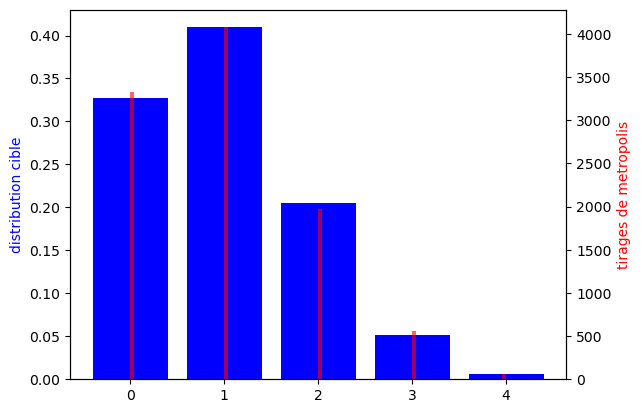
\includegraphics[scale=0.25]{loi bin.png}
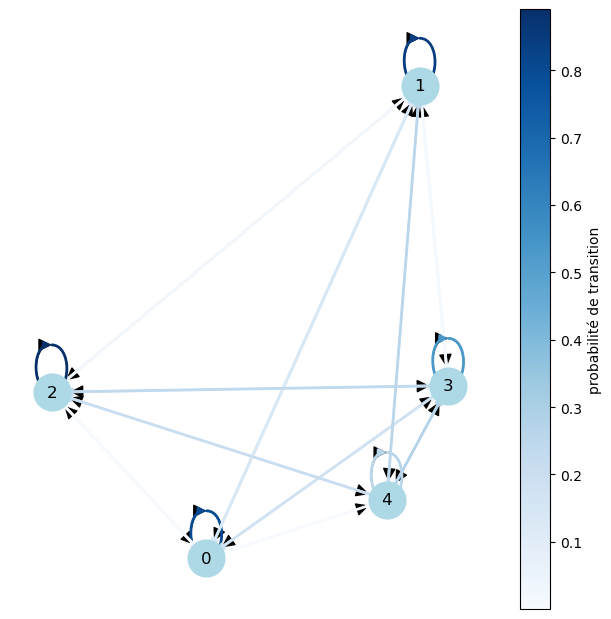
\includegraphics[scale=0.25]{loi bin graph.png}

\newpage
\paragraph{Application à une loi de Poisson:}

\begin{verbatim}
N = 15

distribution_cible = poisson(5)

#matrice de transition uniforme de taille NxN
proposition = np.full((N,N),1/N)

tirage = hasting_metropolis_tirage(0,distribution_cible,proposition,iterations=100_000)
mk_c = markov_chain_from_tirage(tirage,N)
\end{verbatim}

résulats:

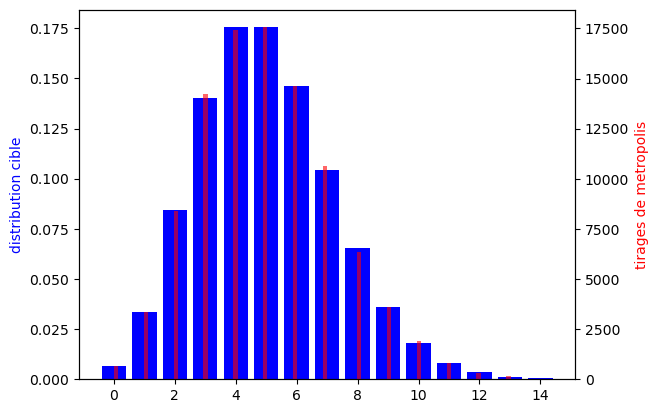
\includegraphics[scale=0.5]{poisson.png}

\newpage
\paragraph{Application à une loi uniform:}

\begin{verbatim}
N = 15

distribution_cible = lambda k : 1/(N-2) if 0<k and k<N else 0

#matrice de transition aléatoire
proposition = np.array([ ligne / ligne.sum()
    for ligne in [np.random.rand(N) for _ in range(N)]
])


tirage = hasting_metropolis_tirage(0,distribution_cible,proposition,iterations=100_000)
mk_c = markov_chain_from_tirage(tirage,N)
\end{verbatim}

résulats:

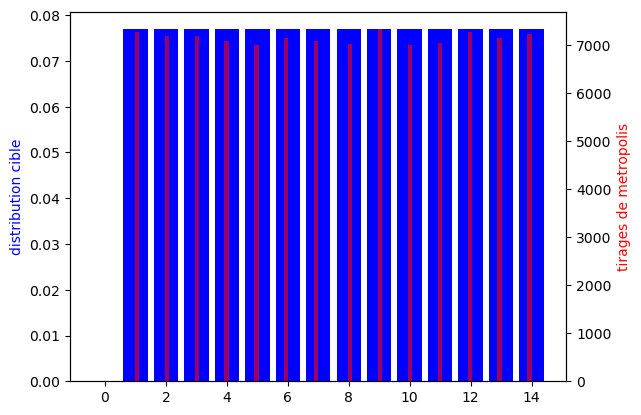
\includegraphics[scale=0.5]{uniforme.png}

\newpage
\paragraph{Application à une loi géométrique:}

\begin{verbatim}
N = 20

distribution_cible = geo(0.33)

#matrice de transition aléatoire
proposition = np.array([ ligne / ligne.sum()
    for ligne in [np.array([abs(np.random.normal(i,1)) for _ in range(N)]) for i in range(N)]
])

tirage = hasting_metropolis_tirage(0,distribution_cible,proposition,iterations=100_000)
mk_c = markov_chain_from_tirage(tirage,N)
\end{verbatim}

résulats:

\includegraphics[scale=0.5]{géometrique.png}

\newpage
\paragraph{Application à une loi quelconque:}

\begin{verbatim}
N = 30

distribution = np.random.rand(N)
distribution = distribution / distribution.sum()

distribution_cible = lambda k : distribution[k] if k < N and 0<=k else 0

#matrice de transition aléatoire
proposition = np.array([ ligne / ligne.sum()
    for ligne in [np.array([abs(np.random.normal(i,1)) for _ in range(N)]) for i in range(N)]
])

tirage = hasting_metropolis_tirage(0,distribution_cible,proposition,iterations=100_000)
mk_c = markov_chain_from_tirage(tirage,N)
\end{verbatim}

résulats:

\includegraphics[scale=0.5]{loi aléatoire.png}


















\newpage

\subsection{Sources}



Documents textuels:
\begin{itemize}
    \item \url{https://fr.wikipedia.org/wiki/Chaîne_de_Markov}
    \item \url{https://dms.umontreal.ca/~bedard/BergeronL_rapport_final.pdf}
    \item \url{https://www.math.univ-paris13.fr/~tournier/fichiers/agreg/2014/cours_markov.pdf}
    \item \url{https://www.math.u-bordeaux.fr/~mchabano/Agreg/ProbaAgreg1213-COURS5-CM.pdf}
    \item \url{https://www.imo.universite-paris-saclay.fr/~pierre-loic.meliot/agreg/markov.pdf}
    \item \url{https://www.college-de-france.fr/fr/agenda/cours/apprentissage-et-generation-par-echantillonnage-aleatoire/algorithme-de-metropolis-hasting}
    \item \url{https://www.math.u-bordeaux.fr/~mibonnef/mimse-markov/recurence-transience.pdf}
    \item \url{https://perso.univ-rennes1.fr/jean-christophe.breton/agreg/AGREG/COURS/ch-mark2.pdf}
    \item \url{https://fr.wikipedia.org/wiki/Processus_stochastique}
    \item \url{https://fr.wikipedia.org/wiki/Méthode_de_Monte-Carlo_par_chaînes_de_Markov}
    \item \url{https://www.math.u-bordeaux.fr/~mchabano/Agreg/ProbaAgreg1314-COURS5-CM.pdf} \\
    \item \url{https://fr.wikipedia.org/wiki/Algorithme_de_Metropolis-Hastings#cite_note-2}
    \item \url{https://www.radcliffe.harvard.edu/news-and-ideas/flash-of-genius} \\
    \item \url{https://fr.wikipedia.org/wiki/Probl\%C3\%A8me_du_voyageur_de_commerce}
    \item \url{https://www.cambridge.org/core/journals/mathematical-proceedings-of-the-cambridge-philosophical-society/article/abs/shortest-path-through-many-points/F1C28B5730B94887F4659FCBF8A1F2BB} % Document de Thomas Kirkman, Jillian Beardwood, J.H. Halton ou John Hammersley.
\end{itemize}

Documents vidéos :
\begin{itemize}
    \item \url{https://www.youtube.com/watch?v=yCv2N7wGDCw}
    \item \url{https://www.youtube.com/watch?v=MxI78mpq_44}
    \item \url{https://www.youtube.com/watch?v=e0ZHDK4DSEI&list=PLWoShwK0FEjovcc32x9LbpDTf8pquPimV}
    \item \url{https://www.youtube.com/playlist?list=PLWoShwK0FEjovcc32x9LbpDTf8pquPimV} \\
\end{itemize}

\end{document}
